\section{Helix Architecture}
\label{sec:arch}
%

Section~\ref{sec:design} describes how \helix lets a DDS specify their model of
operation and then executes against it.  This section presents the \helix system
architecture that implements these concepts.

\begin{figure}
%\fbox{
\begin{minipage}[t]{0.48\textwidth}
%\centering
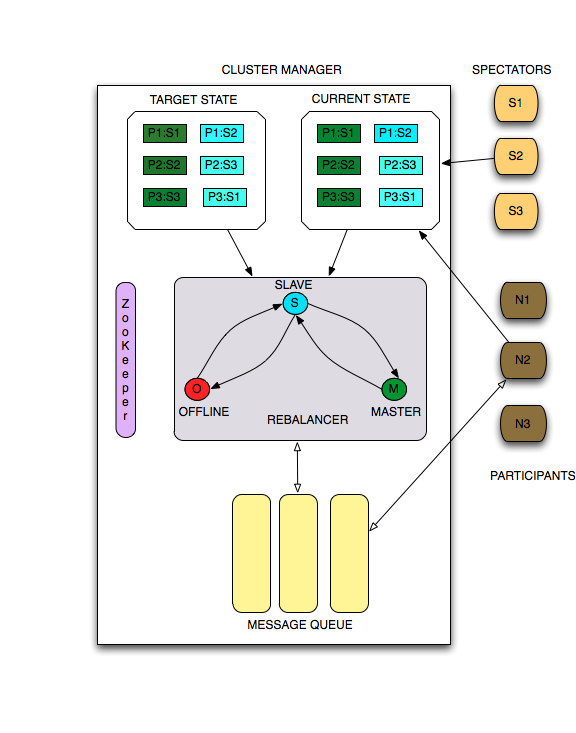
\includegraphics[width=0.95\textwidth]{Helix.png}
%\vspace*{-4ex}
\caption{Helix Architecture}
\label{fig:arch}
\end{minipage}
%}
\end{figure}

\subsection{\helix Roles}
\label{sec:roles}
%
\helix implements three roles, and each component of a DDS takes on at least one of them.
The \emph{controller} is a pure \helix component.  It hosts the state machine engine, 
runs the execution algorithm, and issues transitions against the DDS.  It is the
core component of \helix.

The DDS's nodes are \emph{participants}, but run the \helix library.  The
library is responsible for invoking callbacks whenever the controller initiates
a state transition on the participant.  The DDS is responsible for implementing
those callbacks.  In this way, \helix remains oblivious to the semantic meaning
of a state transition, or how to actually implement the transition.  For
example, in a \emph{LeaderStandby} model, the DDS implements methods
\emph{OnBecomeLeaderFromStandby} \\ and \emph{OnBecomeStandbyFromLeader}.

The \emph{spectator} role is for DDS components that need to observe system
state.  Spectators get notification anytime a transition occurs.  A typical
spectator is the router component that appears in data stores like \\ \ES.  The
routers must know how partitions are distributed in order to direct client
requests and so must be get up-to-date with any partition moves.  The routers do
not store any partitions themselves, however, and the controller never executes
transitions against them.

The roles are at a logical level.  A DDS may contain multiple instances of each
role, and they can be run on separate physical components, run in different
processes on the same component, or even combined into the same process.
 
Dividing responsibility among the components brings a number of key
advantages.  (A) All global state is managed by the controller, and so the DDS can
focus on implementing only the local transition logic.  (B) The participant need
not actually know the state model the control is using to manage its DDS, as long as all the
transitions required by that state model are implemented.  
For example, we can move a DDS from a MasterSlave model to a read-only SlaveOnly
model with no changes to participants.  The participants will simply never
be asked to execute slave$\rightarrow$master transitions.  (C) A
central decision maker avoids the complexity of having multiple components come
to consensus on their roles.    

\subsection{Connecting components with Zookeeper}

Given the three \helix components, we now describe their implementation and how
they interact. \\ Zookeeper~\cite{zookeeper} plays an integral role in this aspect
of \helix.

The controller needs to determine the current state of the DDS and detect
changes to that state, \eg node failures.  We can either build this
functionality into the controller directly or rely on an external component that
itself persists state and notifies on changes. 
When the controller chooses state transitions to execute, it must reliably
communicate these to participants.  Once complete, the participants must
communicate their status back to the controller.  Again, we either build a custom
communication channel between the controller and participants, or rely on an
external system. 
The controller cannot be a single point of failure; in particular, when the
controller fails, we cannot afford to lose either controller functionality or
the state it manages.

\helix relies on Zookeeper to meet all of these requirements.  We utilize
Zookeeper's group membership and change notification to detect DDS state
changes.  Zookeeper is
designed to maintain system state, and is itself fault tolerant.  By storing
all the controller's state in Zookeeper, we make the controller itself stateless
and therefore simple to replace on a failure.  
 
We also leverage Zookeeper to construct the reliable communication channel
between controller and participants.  
The channel is modeled as a queue in Zookeeper and the controller and
participants act as producers and consumers to this queue. Producers can
can send multiple messages through the queue and consumers can process the messages in parallel. 
This channel brings side operational benefits like the ability to cancel
transitions and to send other command messages between nodes.

Figure~\ref{fig:arch} illustrates the \helix architecture and brings together
the different components and how they are represented in Zookeeper.  
The diagram is from the controller's perspective.  The AFSM is specified by each
DDS, but is then itself stored in Zookeeper.  We also maintain the current
states of all partition replicas and target states for partition replicas in
Zookeeper.  Recall that any differences between these states trigger the
controller to invoke state transitions.  These transitions are written to
the messaging queue for execution by the participants.  Finally, \helix
maintains a list of participants and spectators in 
Zookeeper as \emph{ephemeral nodes} that heartbeat with Zookeeper.  If any of
the nodes die, Zookeeper notifies the controller so it can take corrective
action.

\eat{%%%%%%%%%
As shown in Figure ?, We maintain the following state in Zookeeper.

\begin{itemize}
\item \emph{Target State} The target state of a resource in the cluster is stored as a znode in Zookeeper.
\item \emph{Current State} The current state of partitions of the resource on a participant is stored in a znode.
\item \emph{Message Queue} A message queue between the controller and every participant in the cluster is stored in a znode.
\item \emph{Live Instances} Every participant in the cluster creates an ephemeral znode in Zookeeper. This znode gets removed by Zookeeper if the node fails and stopped communicating a heartbeat to Zookeeper.
\end{itemize}

The controller maintains a watch on \emph{Live Instances}, \emph{Target State}, \emph{Current State} and \emph{Message Queue}. It responds to changes in \emph{Live Instances}, \emph{Target State}, \emph{Current State} and executes the state transition algorithm to achieve the \emph{Target State} of the cluster.

For example, when a new node is added to the cluster, Helix recomputes the \emph{Target State} of the cluster to assign some of the partitions on to the new node. Once the \emph{Target State} is specified, the controller is notified and it computes the state transitions to go from \emph{Current State} to \emph{Target State}. After applying the constraints defined on the state model and optimization goals, a  subset or all of the state transitions are then enqueued into the \emph{Message Queue} of the appropriate participant nodes. The participants watch their \emph{Message Queue} for messages from the controller. The Helix library in the participant invokes the callbacks supplied by the DDS that correspond to the state transitions. Once the callbacks complete successfully, the Helix library in the participant updates the \emph{Current State}.
}%%%%%%%%%%%%%

\subsection{DDS Integration with \helix}
This section describes how a DDS deploys with \helix.
The DDS must provide 3 things.

\noindent \textbf{Define Cluster}
The DDS defines the physical cluster and its physical nodes.  \helix provides an
admin API, illustrated here: 
\small\begin{verbatim}
helix-admin --addCluster EspressoCluster 
helix-admin --addNode EspressoCluster <esp10:1234>
\end{verbatim}
\normalsize

\noindent \textbf{Define Resource, State Model and Constraints}
Once the physical cluster is established, the next step is to logically add the
DDS, including the state model that defines it and the resources it will supply.
Again, \helix provides an admin API: 
\small\begin{verbatim}

  helix-admin --addStateModel MasterSlave states=<M,S,O> 
              legal_transitions=<O-S, S-M, M-S, S-0> 
              constraints="count(M)<=1 count(S)<=3" 
  helix-admin --addResource 
             clusterName=EspressoCluster
		     resourceName=EspressoDB numPartitions=8 
		     replica=3
		     stateModelName=MasterSlave
\end{verbatim}
\normalsize


Given the above admin commands, \helix itself computes an initial target state
for the resource: 
\small\begin{verbatim}
{
  "id" : "EspressoDB",
  "simpleFields" : {
    "IDEAL_STATE_MODE" : "AUTO",
    "NUM_PARTITIONS" : "8",
    "REPLICAS" : "1",
    "STATE_MODEL_DEF_REF" : "MasterSlave",
  },
  "mapFields" : {
    "EspressoDB_0" : { "node0" : "MASTER",
                       "node1" : "SLAVE"  },
    "EspressoDB_1" : { "node0" : "MASTER",
                       "node1" : "SLAVE"  },
    "EspressoDB_2" : { "node0" : "SLAVE",
                       "node1" : "MASTER" },
    "EspressoDB_3" : { "node0" : "SLAVE",
                       "node1" : "MASTER" },
  }
}
\end{verbatim}
\normalsize

\noindent \textbf{Implement Callback Handlers}
The final task for a DDS is to implement logic for each state transition encoded
in their state machine.  We give a partial example of handler prototypes for
\ES's use of MasterSlave.

\small\begin{verbatim}
EspressoStateModel extends StateModel
{
 void offlineToSlave(Message task,
     NotificationContext context)
 {
  // DDS Logic for state transition
 }
 void slaveToMaster(Message task,
     NotificationContext context)
 {
  //DDS logic for state transition
 }
}
\end{verbatim}
\normalsize
\subsection{Scaling \helix into a Service}

\eat{%%%%%%%%
We carefully divided up \helix's responsibilities
between the controller and participant roles and, in doing so, gain a number of
advantages.

\begin{itemize}

\item  The participant remains completely unaware of the DDS's
global state.   This makes the job of developers implementing the DDS specific
logic considerably simpler; they only need to write the node's local transition
logic. The responsibility of maintaining the distributed system and responding
to changes in that global state is solely with the controller, which DDS
developers need not touch.
 
\item Since the participant is unaware of global state is
that the same DDS can easily be configured differently for different use cases.
Consider key-value storage systems, which typically support reads and writes,
but sometimes are deployed as read-only (with data periodically bulk loaded).
In the former case, we might use a MASTER-SLAVE state model, and in the latter,
a MASTER-only (or SLAVE-only) mode, since there is no need to differentiate
replicas.  In both cases, the participant code does not change, and the
participants are in fact oblivious to what state model is invoked. 

\item Having a central controller component with global system state simplifies
transition decision-making.  An alternative approach followed by many distributed systems
is to divide responsibility for decisions among the participants.  Consider the
LeaderStandby state model.  A single participant per partition serves as Leader
at any given time.  In the absence of a controller, participants use a central
lock manager to coordinate leader election; when the current leader fails, the
first participant to acquire the lock becomes the new leader.  In large systems with many partitions
this can lead to a herd effects that can be detrimental to performance. 

\item Multiple participants simultaneously making decisions based on global state increases the chance of \emph{Split Brain} problem where multiple participants make conflicting decisions about the global state of the cluster.

\end{itemize}
}%%%%%%%%%

%\subsubsection {Scaling the controller}
The risks of having a single controller as we have described so far is that it
can become a bottleneck or a single source of failure (even if it is easy to
replace).  We now discuss our approach for distributing the controller that
actually lets Helix provide cluster management as a service. 

To avoid making the controller a single point of failure, we deploy multiple
controllers. A cluster, however, should be managed by only one controller at a time. 
This itself can easily be expressed using a LeaderStandby state model with the constraint 
that every cluster must have exactly one controller managing it! Thus we set up multiple 
controllers as a participants of a \emph{supercluster} comprised of the different clusters 
themselves as the resource. One of the controllers manages this supercluster. If that controller 
fails, another controller gets selected as the Leader for the supercluster. This
guarantees that each cluster has exactly one controller.  

The supercluster drives home \helix's ability to manage any DDS, in this case
itself.  \helix itself becomes a scalable DDS that in turns manages multiple DDSs. 
In practice we typically deploy a set of 3 controllers capable of managing over
50 clusters. 

\eat{%%%%%%%%%
\subsection{OLD STUFF FOR ARCH, BUT CAN PULL TEXT FROM HERE}

\subsection{Supporting no SPOF}
In order for to support this abstraction we need a communication
channel between controller and participant. Its also important that
controller does not become a Single Point Of Failure (SPOF) and
system is stable if any of the component in the system fails. This
means that the state of the system must be durable and also the
communication channel between controller and participant must be able
to handle failures. We use Zookeeper to maintain the state
of the system. Along from being highly available system to store the
cluster state Zookeeper also provides group member ship and also
change notification in cluster state. More info on Zookeeper can be
found at \url{http://zookeeper.apache.org}

\subsection{Stabilizing the system---This should be taken care of by design
section...delete this later}

External changes (Section~\ref{Requirements}) conspire to change the
state of the system, potentially into a less desirable one. The job of
the controller is to restore balance. It does so by defining
\be
\item Current State (CS) --- the current state of the system. The example of
Table~\ref{CS_Example} describes a system with 3 nodes, \(N_1, N_2,
  N_3\), and 4 partitions
such that partition 1 has a replica 
(i) in state \(M\) on \(N_1\)
(ii) in state \(S\) on \(N_2, N_3\)
(iii) in state \(O\) on \(N_4\)
\item Ideal State (IS) --- the final expected state of partition on a 
node. It is re-calculated every time there is a change in the system.  
This is not expressed in terms of an assignment as in
Table~\ref{CS_Example}. Instead, it is expressed in terms of desiderata.
In the example of Espresso (Section~\ref{Espresso}), 
  \be
  \item A partition should not have 2 replicas on the same machine
  \item The maximum number of partitions in state \(M\) on any machine
  should be minimized
  \item \TBC
  \ee
\ee

\begin{table}
\centering
\begin{tabular}{|l|l|l|l|l|} \hline \hline
            & \(N_1\) & \(N_2\) & \(N_3\) & \(N_4\) \\ \hline \hline
State \(M\)       & \(P_1\)  &         &         & \\ \hline 
State \(S\)       &         & \(P_1\) & \(P_1\) & \\ \hline 
State \(O\)       &         &         &         & \(P_1\) \\ \hline 
\end{tabular}
\label{CS_Example}
\caption{Example of Current State}
\end{table}

\subsubsection{Instantiating an IS}
We take the requirements of an IS as input and produce a mapping of X to
Y as an output.

%{\em 
The goal of this algorithm is simple, it
considers all the nodes that are currently up in the cluster and
computes the state for each partition on a given node so that cluster
is stable and all the constraints are satisfied.


Consider a partition and 4 nodes. 
Lets take a simple example of having these constraints.  Number of
partitions 3. Number of nodes 3 Add the example here and compute the
ideal state such that constraints are satisfied. A simple solution is
N1:M N2:S N3:S

Now lets walk through what happens when the nodes are started in the
cluster.

All nodes(N1,N2,N3) start in the Offline state, the ideal state based
on the constraint and live nodes is computed as N1:MASTER, N2:SLAVE,
N3:SLAVE. Another key aspect of the algorithm is parallelize the
transitions without compromising the state constraints. More details
on this algorithm can be found in section

Controller sends OFFLINE-SLAVE transition message to all 3 nodes, as
soon N1 becomes SLAVE, controller issues SLAVE-MASTER transition
message to N1. It wont issue any more transitions after N1 becomes
master because all the constraints of the system are satisfied. Note
that all transitions are issues by consulting the state machine
provided by the application.

Failure:

We will see how the same algorithm is applicable to a Node Failure.
Lets say node N1 fails, then controller re computes the Idealstate as
N2:M, N3:S. Note that controller knows that N1 is down and assigns
MASTER state to N2.  The current state immediately after the failure
is N1:O, N2:S N3:S. It issues S-M transition to N2.

Similarly Node addition, removal and partition addition/removal are
also taken care of in similar fashion.


The role of a spectator is simply be aware of the state changes
happening in the cluster.

Algorithm: Psuedo code Controller gets the Ideal State and the Current
State of active storage nodes from ZK Compute the delta between Ideal
State and Current State for each partition across all participant
nodes For each partition compute tasks based on State Machine
Table. Its possible to configure priority on the state Transition. For
example in case of Espresso, Attempt Mastership transfer if possible
without violating constraint.  Partition Addition Drop Partition[Can
be done when its the only task possible per partition to avoid
complexity] Add the transitions[parallel if possible] to respective
queue for each node.  If a task is dependent on another task being
completed do not add that task.  After any task is completed by
Participant, Controllers gets notified of the change and State
Transition algorithm is re-run until the current state is same as
Ideal State.

Apart from satisfying the state constraints the same algorithm also
takes care of satisfying the constraints on state transition
}%%%%%%%%%%%%


